\chapter{SYSTEM}
\label{systemChapter}
The goal of the proposed visual analytic system is to enable analysts to simulate the first- and second-order effects of climate events to the food trade network. Identification of the effects, along with potentially vulnerable countries, can be used by policy makers and international aid managers. For instance, in the event of a drought in Argentina, analysts would be able to use the framework to determine which countries would likely be impacted the most. They could then advise international aid managers to begin staging supplies near the predicted areas.\par
\section{Data, Assumptions, and Formulas}
\label{daf}
	The Food and Agriculture Organization (FAO) of the United Nations (UN) Statistics Division maintains the Food and Agriculture Organization Corporate Statistical Database (FAOSTAT). This database provides free access to food and agriculture data for over 245 countries and territories and covers all FAO regional groupings from 1961 to the most recent year available (\cite{faostat}).\par
	The data in this thesis is a snapshot from the FAOSTAT database containing trade link data for the years 1986 through 2013. The FAOSTAT database contains a reporting country, a partner country, the type (i.e. import or export), the trade year, the trade good and dollar value. A country will report the value of a particular good it imported for that year from the partner country. That partner country also reports the exporting value. Since these two reports are not always the same, as seen in Table \ref{faotableLinks}, some preprocessing is required.\par
	\begin{center}
		\begin{table}[htb]
			\begin{tabular*}{\textwidth}{@{\extracolsep{\fill}}|l|l|l|l|l|l|}
				\hline
				Trade Year&Reporter&Partner&Type&Item&Value\\
				\hline
				2011&USA&Japan&Maize&Export&{\$3,831,683,000}\\ \hline
				2011&Japan&USA&Maize&Import&{\$4,818,714,000}\\ \hline
			\end{tabular*}
			\caption[SAMPLE FAOSTAT DATA]{Sample FAOSTAT data}
			\label{faotableLinks}
		\end{table}
	\end{center}\par
	Since the FAOSTAT database contains two sets of data, the importing country's reported data and the exporting country's reported data, preprocessing was done to merge the two reported values. The processed trade links are then defined by the exporting country, the importing country, the trade year, the trade good and the dollar value of the trade link. Some example links are shown in Table \ref{tableLinks}. Bilateral trade associations and triad constructions were calculated and stored in our database.\par
	\begin{center}
		\begin{table}[htb]
			\begin{tabular*}{\textwidth}{@{\extracolsep{\fill}}| l | l | l | l | l |}
				\hline
				Trade Year & Exporter & Importer & Item & Value \\
				\hline
				2011 & USA & Japan & Maize & {\$4,325,199,000} \\ \hline
				2011 & Poland & Sweden & Molasses & {\$2,648,000} \\ \hline
				2011 & Afghanistan & Australia & Almonds shelled & {\$13,000} \\ \hline
			\end{tabular*}
			\caption[SAMPLE TRADE LINKS COMPRISING THE INTERNATIONAL FOOD TRADE NETWORK]{Sample trade links comprising the international food trade network}
			\label{tableLinks}
		\end{table}
	\end{center}\par
	To model the cascading effects of a climate event a simulation engine was created. In construction of the simulation engine we made the following assumptions. First, for the simulation of a climate event, the trade link value for all the selected country's export links is reduced. For instance, if a 10\% reduction in wheat exports is simulated from a country, every export trade link is reduced by 10\%. Second, the reduction percentage is a reduction of export links and not a reduction of production. This is important because if a production reduction is assumed it could potentially decrease the export trade links by a larger amount than the specified reduction for the country to maintain its own stores of the trade good. Another benefit is that we are able to model indirect export reductions, such as export restrictions. Third, the export links will all be reduced regardless of outside influences. There is no favoritism in the decision making of which export trade links to reduce; that is, there is an equal reduction in trade goods to all trading partners. Lastly, the reduction in imports to a country is then extrapolated to its own export trade links. The country is calculated to lose that value of goods and will first reduce its own exports to mitigate the loss of imports. Such assumptions pose the risk of an overly simplistic export reduction formula which may not be realistic, however we believe that it does offer a good starting point.\par
	The vulnerability index to a country is then defined as 
	\begin{equation} \label{vulnerability}
		v=\frac{\sum _I - \sum _{I_\Delta}}{\sum _I + \sum _E}
	\end{equation}
	where $\sum _I$ is the sum of the country's import trade links dollar values before the simulation reduction, $\sum _{I_\Delta}$ is the sum of all of the country's import trade link dollar values after the simulation reduction and $\sum _E$ is the sum of all of the country's export trade link dollar values before the simulation reduction. Note that denominator is the sum of both import and export trade link dollar values. Again, we make the assumption that a country would reduce its exports to overcome the loss of imports.The range of values is 0 to 1 and a higher number indicates a higher vulnerability. If a country does not suffer any import reduction, that is $\sum _{I_\Delta}=\sum _I$, then the vulnerability index will be 0: $v=0$. If a country loses its entire import portfolio, that is $\sum _{I_\Delta}=0$, the vulnerability index is then a function of the value of its ratio of its imports and exports: $\frac{\sum _I}{\sum _I + \sum _E}$. If that country does not have any export links, that is $\sum _{E}=0$, then the vulnerability index is a function of the value of lost imports: $\frac{\sum _I - \sum _{I_\Delta}}{\sum _I}$. If a country does not have any export links and loses its entire import portfolio, that is $\sum _{E}=0$ \& $\sum _{I_\Delta}=0$, then the vulnerability index will be 1: $v=1$.\par
	Another index used in the system is import dependence, defined as 
	\begin{equation} \label{importRatio}
	d_l=\frac{l}{\sum _I + \sum _E}
	\end{equation}
	where $l$ is the dollar value of the trade link and $\sum _I$ is the sum of the all of the country's import trade link dollar values and $\sum _E$ is the sum of the all of the country's export trade link dollar values. The higher the number the higher the import dependency of the trade link. Note that denominator is the sum of both import and export trade links. Again, we make the assumption that a country would reduce its exports to overcome the loss of imports.
	\section{System Architecture}
		The proposed visual analytics system is a web-based system consisting of a front-end website for user display and interaction and a back-end system for data retrieval. The system is accessible from a modern web browser and was developed with an HTML front-end utilizing JavaScript for advanced features. The core of the visualization was created by an open-source JavaScript library called Data-Driven Documents (D3), \citep{d3}. This is a JavaScript library providing many mechanisms for manipulating document object model (DOM) elements based on data. A powerful concept which was utilized extensively was selections. This allows attribution of an array of data to an element, usually a DIV. Then child nodes are created, updated, and destroyed based on changes to the array. This mechanism allowed a extremely large dataset to be held in memory. The benefits of this are two-fold; efficient manipulation of the dataset resulting in responsive visualizations and reducing the need for numerous database calls limiting the effect of network latency.\par
		Connecting the front-end to the back-end are RESTful APIs. The APIs exist on the back-end web servers to connect to a database and provide the data to the front-end. These APIs were written in Java and utilize a mechanism to execute simple transactional-SQL queries. The data is then returned in a D3 friendly arrayed JavaScript Object Notation (JSON) formatted object for processing in the front-end.\par
	\section{Visual Analytics Framework}
		A diagram of the visual analytic framework is shown in Figure \ref{architecture}. The three parts of the system are the data, the model and the visualization. In my system the data is the database and supplemental data as described in Section \ref{daf}. The model part of the system is accomplished by modeling the trade links as a network graph and calculation of vulnerability indices, triad z-scores and import dependencies. These calculations are described in more detail in the following sections. The visualization graphically represents the data and models to allow for analysts to visually detect patterns. The feedback loop is made up of the action and finding boxes on the right side of Figure \ref{architecture}.\par
		My framework allows for a domain expert to simulate a climate event to explore the first- and second-order effects to the international food trade network and identify any potentially vulnerable countries. After a subset of data is selected, a simulation is modeled and the visualization displays the effects. Further filtering and interactions, such as panning and zooming, in the feedback loop allow for enhanced pattern recognition.\par
		\begin{figure}[htb]
			\center{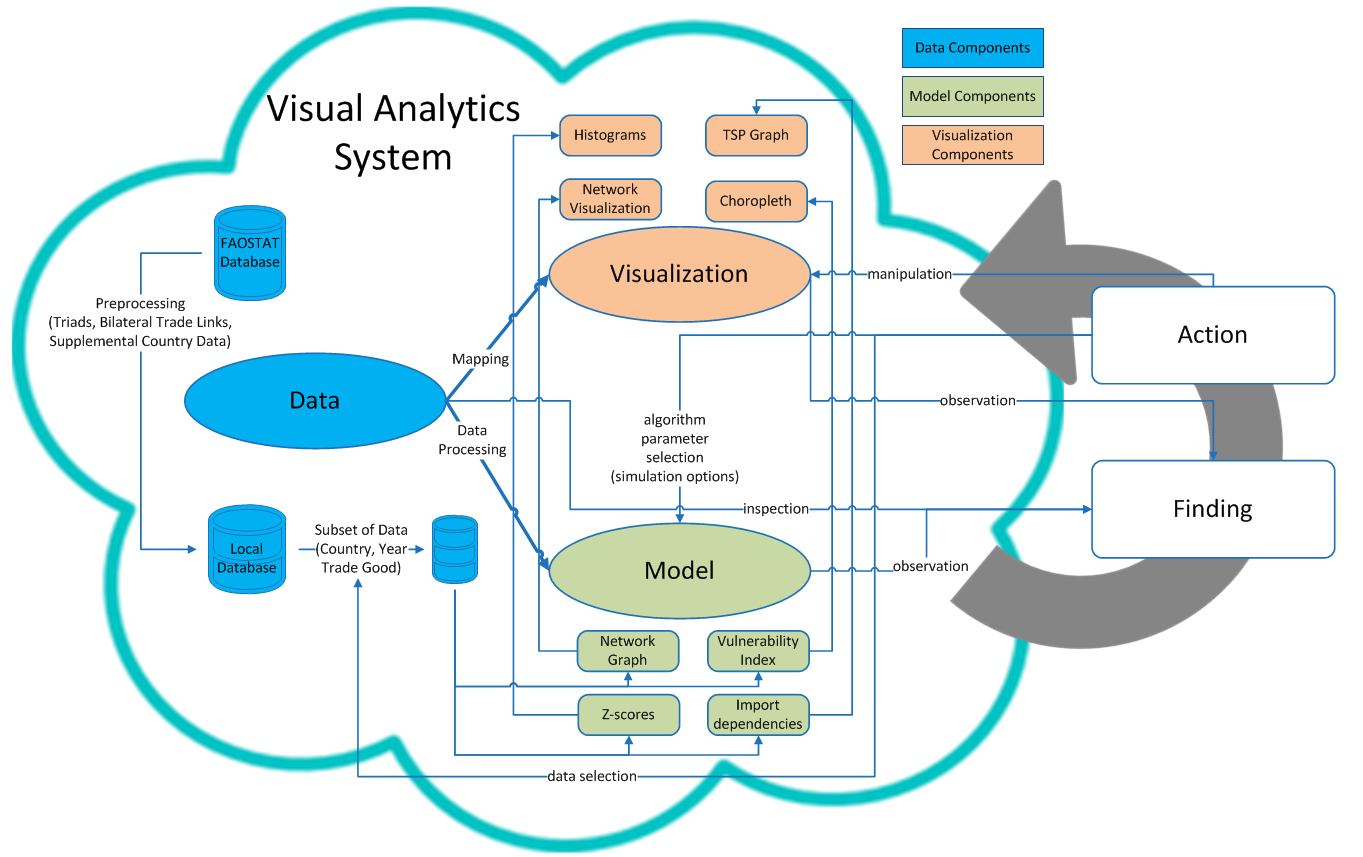
\includegraphics[width=\textwidth]{figures/va_system.png}}
			\caption[VISUAL ANALYTICS SYSTEM DIAGRAM]{Visual Analytics System diagram, (motivated by \cite{sacha2014knowledge})}
			\label{architecture}
		\end{figure}
		The main visualization of the visual analytic system is a dashboard (Figure \ref{dashboardSections}). In the top left part of the dashboard a combo box exists so the user may select the year to analyze. The rest of dashboard is composed of 5 distinct sections as seen in Figure \ref{dashboardSections}. The histogram charts in Figure \ref{dashboardSections}-1 shows the distribution of trade links based on the import dependency for four staple crops, with the most opaque indicating the currently selected crop. Figure \ref{dashboardSections}-2 shows the network graph, a visual representation of the food trade network, and all of the import and export trade links of the currently selected crop. Figure \ref{dashboardSections}-3 is the choropleth map which visualizes the impacts of the simulated climate event from Figure \ref{dashboardSections}-5. Both the network graph and choropleth map allow for a user to select a country for the simulation by clicking on the node in the graph or country on the map. The selected country is then given a dark border in both views as seen in Figures \ref{networkGraph} and \ref{map}. Figure \ref{dashboardSections}-4 shows the normal triad significance profile (TSP) graph based on four staple crops for the year 2013 overlayed with the TSP graph of the currently selected data subset. Figure \ref{dashboardSections}-5 shows the parameters for the climate event simulation engine. In each of the sections moving the mouse over pertinent parts of the visualizations displays a tooltip for displaying detailed information, as in Figure \ref{tooltip}. This tooltip displays the trade link data from a link of the 2013 wheat network graph. In 2013 Egypt imported \$576 million dollars which accounted for 23\% of total Egyptian wheat imports and 11\% of the total Egyptian imports of four staple crops.\par
		\begin{figure}[htb]
			\center{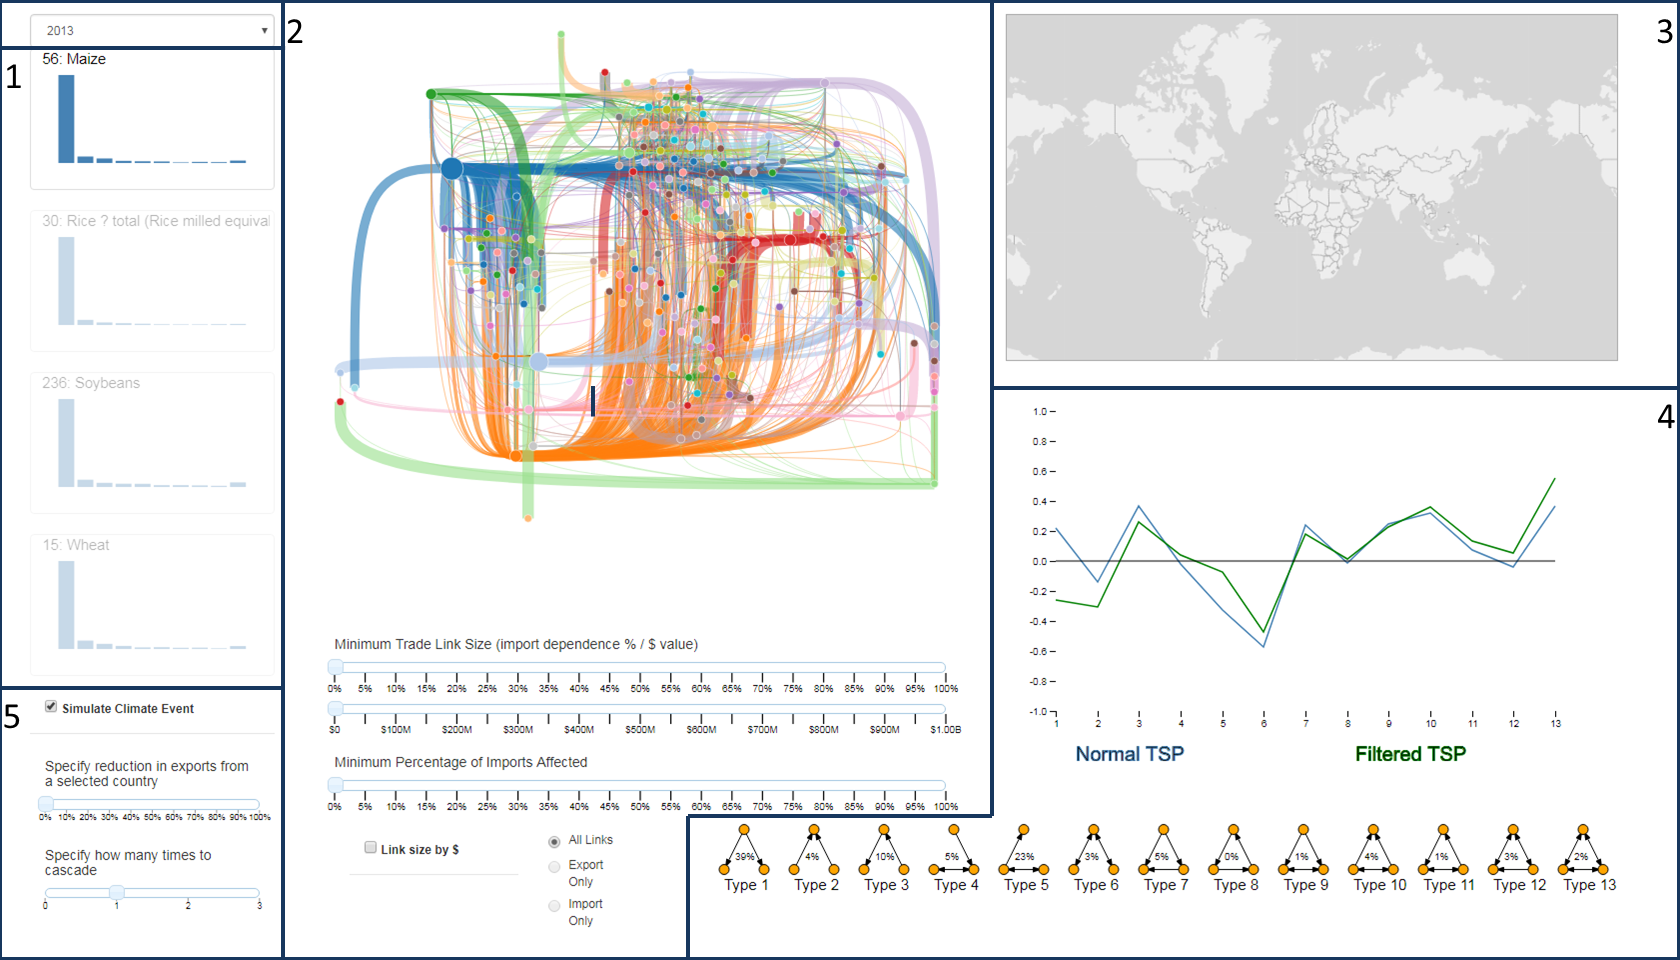
\includegraphics[width=\textwidth]{figures/sections.png}}
			\caption[SECTIONS OF THE DASHBOARD]{Sections of the dashboard. 1: Histograms of trade link import dependencies grouped by crop; 2: Network graph and filtering options; 3: A choropleth map visualizing the impacts of a simulated climate event; 4: Triad significance profile graph; 5: Climate event simulation engine parameters.}
			\label{dashboardSections}
		\end{figure}
		\begin{figure}[htb]
			\center{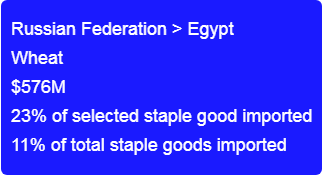
\includegraphics[width=150px]{figures/tooltip.png}}
			\caption[TOOLTIP OF A LINK IN THE NETWORK GRAPH]{A tooltip is displayed when the user moves their mouse over pertinent parts of the visualizations. In this example a tooltip displays the trade link data from a link of the 2013 wheat network graph. The tooltip shows the trade link values for that year. In 2013 Egypt imported \$576 million dollars which accounts for 23\% of Egyptian wheat imports and 11\% of the total Egyptian imports of four staple goods.}
			\label{tooltip}
		\end{figure}
		\subsection{Simulation Option (Figure \ref{dashboardSections}-5)}
			The simulation of climate events is the defining part of the system. This section allows for the parameters for the climate event simulation to be defined. The first checkbox in Figure \ref{dashboardSections}-5 indicates whether we want the simulation engine to run or not. The calculations for the simulation engine are time consuming so generally this is only checked after an interesting scenario is identified. The other controls in Figure \ref{dashboardSections}-5 only appear if the checkbox is checked and the choropleth map (Figure \ref{dashboardSections}-4) will only be colored in if a simulation is being ran.\par
			The slider in the next part of Figure \ref{dashboardSections}-5 indicates the total percentage of reduction in export links to simulate. The last slider in Figure \ref{dashboardSections}-5 indicates how many times the reduction should cascade down. Cascading zero times implies that only the selected country's direct importers are affected. Addition of the first cascade level will add the second-order effects of trade link disruption to the initial importer's export partners.\par
		\subsection{Histograms (Figures \ref{dashboardSections}-1, \ref{histogram})}
			The histogram charts in Figure \ref{dashboardSections}-1 show the distribution of trade links, based on import dependency (Equation \ref{importRatio}), for each of the four staple crops. The trade links are binned in increments of 10 percent. The first group is 0 to 10\%, the next 10 to 20\%, et cetera. The more opaque histogram chart indicates the currently selected good and clicking on any of the other histograms changes the selected good to the clicked chart. The y-axis of the histogram shows the quantity of trade links in each bin and the x-axis is the import dependency. For example, the furthest right bin represents the trade links which account for 90 to 100\% of the importing country's entire import portfolio of the trade good. The tooltips (example in Figure \ref{histogram}) in this section show the number of trade links in a bin and the top 10 trade links by dollar value. The trade link data shown on the tooltip is the exporting country, the importing country, the dollar value and the import dependency.\par
			\begin{figure}[htb]
				\center{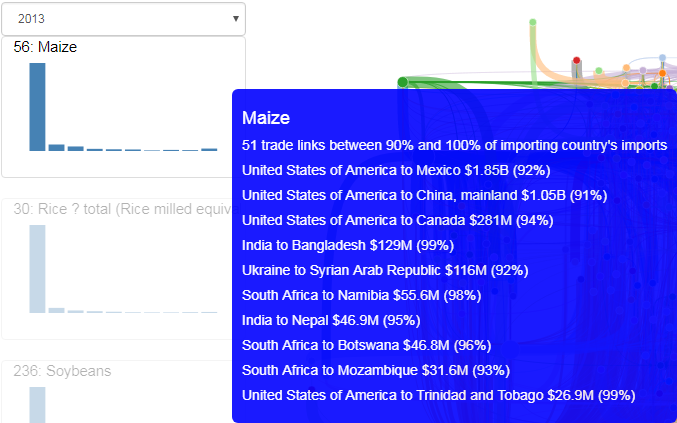
\includegraphics[width=\textwidth]{figures/histogram.png}}
				\caption[HISTOGRAM FOR CORN IN 2013]{A zoomed in view of the histogram for corn in 2013, with the tooltip showing information for the last bin. The trade links are binned into groups based on their percentage contribution to the importing country's total imports of that product. This can be used to quickly identify countries who have a large dependency on a singular trade link. The tooltip here shows that, in 2013, Mexico's import of corn was almost exclusively (92\%) from the United States at a trade value of \$1.85 billion.}
				\label{histogram}
			\end{figure}
			Generally, links in the left-most bins indicate more diversified imports and the right-most indicate imports that are made up of fewer trade links. This can be used to quickly identify countries that have a large dependency on a single trade link. As international food trade grows identification of reliance on imports is important to identification of vulnerability. Results from \cite{d2016teleconnected} and \cite{gephart2016vulnerability} suggest that diversification of trade partners reduce food security risks.\par
			An example is present in Figure \ref{histogram}. The presence of bins in the far right group in the histograms for corn (Figure \ref{histogram}) indicate that there is a large dependency for some countries on a single trade link. Mousing over the last bin and displaying the tooltip (Figure \ref{histogram}, tooltip) shows that in 2013 Mexico relied on the United States for about 92\% of its corn. Domain experts would be able to associate these types of links to potential areas of concern. If the importing country also exports we have the potential for the appreciation of cascading effects. By looking at bins that are in the at-risk group (furthest right in Figure \ref{histogram}) we can hover over the histogram and view the trade link information and corresponding import dependency. In this way the histograms can be used to select a country in the network graph or on the map as a starting point for exploration.\par
			With a country selected (e.g. Mexico) analysts would be able explore further questions such as: if a climate event affected the United States in a manner that was significant enough to prompt the United States to stop shipping corn to Mexico, even temporarily, what cascading effects do we see? Are any countries dependent on imports from Mexico? We are able to visualize these first- and second-order effects in the network graph and choropleth map.\par
		\subsection{Network graph (Figure \ref{networkGraph})}
			\begin{figure}[htb]
				\center{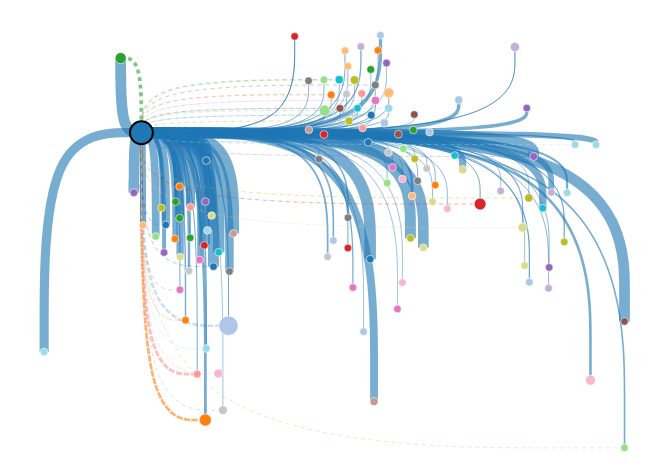
\includegraphics[width=\textwidth]{figures/networkGraph.png}}
				\caption[NETWORK GRAPH OF 2013 CORN IMPORTS AND EXPORTS FROM THE UNITED STATES]{A network graph showing all the corn that was imported or exported to the United States in the year 2013. The selected country is indicated by the dark outline of the node, in this case the United States (large blue dot on the left side). Node size is a function of the total GDP of the country. Solid lines indicate export trade links from the selected country if applicable. Dashed lines indicated import trade links to the selected country. Depending on the option selected the thickness of the trade links indicate the trade link's contribution to the importing country's total staple good imports or the trade link's dollar value.}
				\label{networkGraph}
			\end{figure}
			The international food trade market can naturally be represented by a weighted directed network graph as in Figure \ref{networkGraph}. Nodes of the graph are countries involved in trade and the edges are the trade links associated with the two countries. The node size is a function of the total GDP of the country. Node color is arbitrary but is constant for the life of the visualization. The nodes are positioned close to geographically correct with some perturbations for visual readability. Direction is indicated by color, the edge takes the color of the exporting country. For instance in figure \ref{networkGraph} the United States is blue and all export links from the United States are colored blue. Import links to the United States take the color of the exporting country, as. In the default view the weight of the link is the import dependency (Equation \ref{importRatio}) of the trade link. The weight of the link is indicated by the thickness of the line representing the edge. There is also an option (Figure \ref{networkGraphOptions}) to display the link size by dollar value. If no country is selected solid lines indicate both import and export trade links. If a country is selected its node will have a dark outline as in Figure \ref{networkGraph}. The large blue dot on the left side of the graph shows the selected country, in this case the United States. The edges are represented by solid lines, indicating export trade links from the selected country, and dashed lines, indicating import trade links to the selected country. If a climate event is being simulated alternating dashes and spaces indicate a link broken by the export reduction of the simulation. \par
			The three sliders in this section (Figure \ref{networkGraphOptions}) filter the network graph. The first slider in Figure \ref{networkGraphOptions} hides any trade links that have an import dependency of less than the selected value. This is used to potentially filter out insignificant trade links, e.g. accounting for 1\% of a country's total imports. The second slider filters out any trade links whose raw dollar value is not at least the selected value. Again this can be used to filter out insignificant links such as a trade link of \$1,000 dollars. The third slider is only visible in simulation mode and is used to filter out nodes whose total imports are affected by at least the slider's current value. This is useful for determining which countries are significant affected, including cascading effects, by the simulated climate event. The single checkbox will show the links weighted by dollar value instead of the import dependency (Equation \ref{importRatio}). The group of radio buttons will determine which type of links are shown. This is only available when a country is selected and not in simulation mode. There is also behavior for panning, zooming and node repositioning to facilitate interaction.\par
			\begin{figure}[htb]
				\center{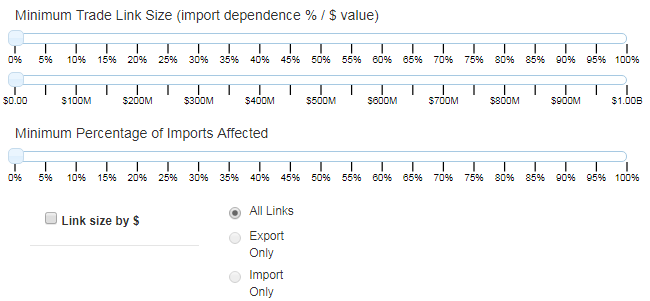
\includegraphics[width=\textwidth]{figures/networkGraphOptions.png}}
				\caption[OPTIONS FOR FILTERING AND DISPLAY OF THE NETWORK GRAPH]{Options for filtering and display of the network graph. The first slider hides any export trade links that contribute less than the selected value to the link's importing country's total import value of the trade good. The second slider filters out any trade links whose raw dollar value is not at least the selected value. The third slider is only visible in simulation mode and is used to filter out nodes whose imports are affected by at least the slider's current value. The single checkbox will show the links weighted by dollar value instead of the import dependency (Equation \ref{importRatio}). The group of radio buttons will determine which type of links are shown. This is only available when a country is selected and not in simulation mode.}
				\label{networkGraphOptions}
			\end{figure}
			The network graph is used to visualize trade links in the international food trade network. As risk is a function of import dependency the thickness of the link indicates the importance of that trade link to the importing country. Selecting a country here will filter the data to only include exports from and imports to the selected country. It is also required for any climate simulation as we need to define the country who will have their exports reduced.\par
			Continuing on the example from above, Mexico is the selected country and the trade links to and from Mexico are inspected. The tooltip for the link in the network graph (Figure \ref{mexicoMiddleMan}, tooltip) shows that although the trade link provides approximately 92\% of the corn imported to Mexico (from the histogram), it only accounts for about 37\% of the total imports of staple goods. This percentage can be used by a domain-expert to gauge the diversity of imports across the staple goods of the importing country to further evaluate the level of vulnerability. \par
			With a country selected analysts would also be able to see trade links upstream of a country. An example of this is in Figure \ref{mexicoMiddleMan}-2. Mexico is the selected country (purple) and the network graph is showing corn trade links for 2013, with trade links filtered by import dependencies of 25\% and dollar values of at least \$250 million. This has the effect of showing only the more significant trade links to and from Mexico. The large dashed line, indicating an import trade link, into Mexico shows that Mexico is highly dependent on the United States for a large portion of its corn (92\% from \ref{mexicoMiddleMan}-1, tooltip). The solid line, indicating an export link, out of Mexico shows that Venezuela is moderately dependent on Mexico for corn (29\% from \ref{mexicoMiddleMan}-2, tooltip). This would aid to identify countries that act as middle men, countries that also export the good they import. These countries' export partners are more susceptible to cascading effects due to climate events affecting their supply partner. This is especially true if the middle man has a high dependency on a single trade link as in this example of Mexico and the United States.\par
			\begin{figure}[htb]
				\center{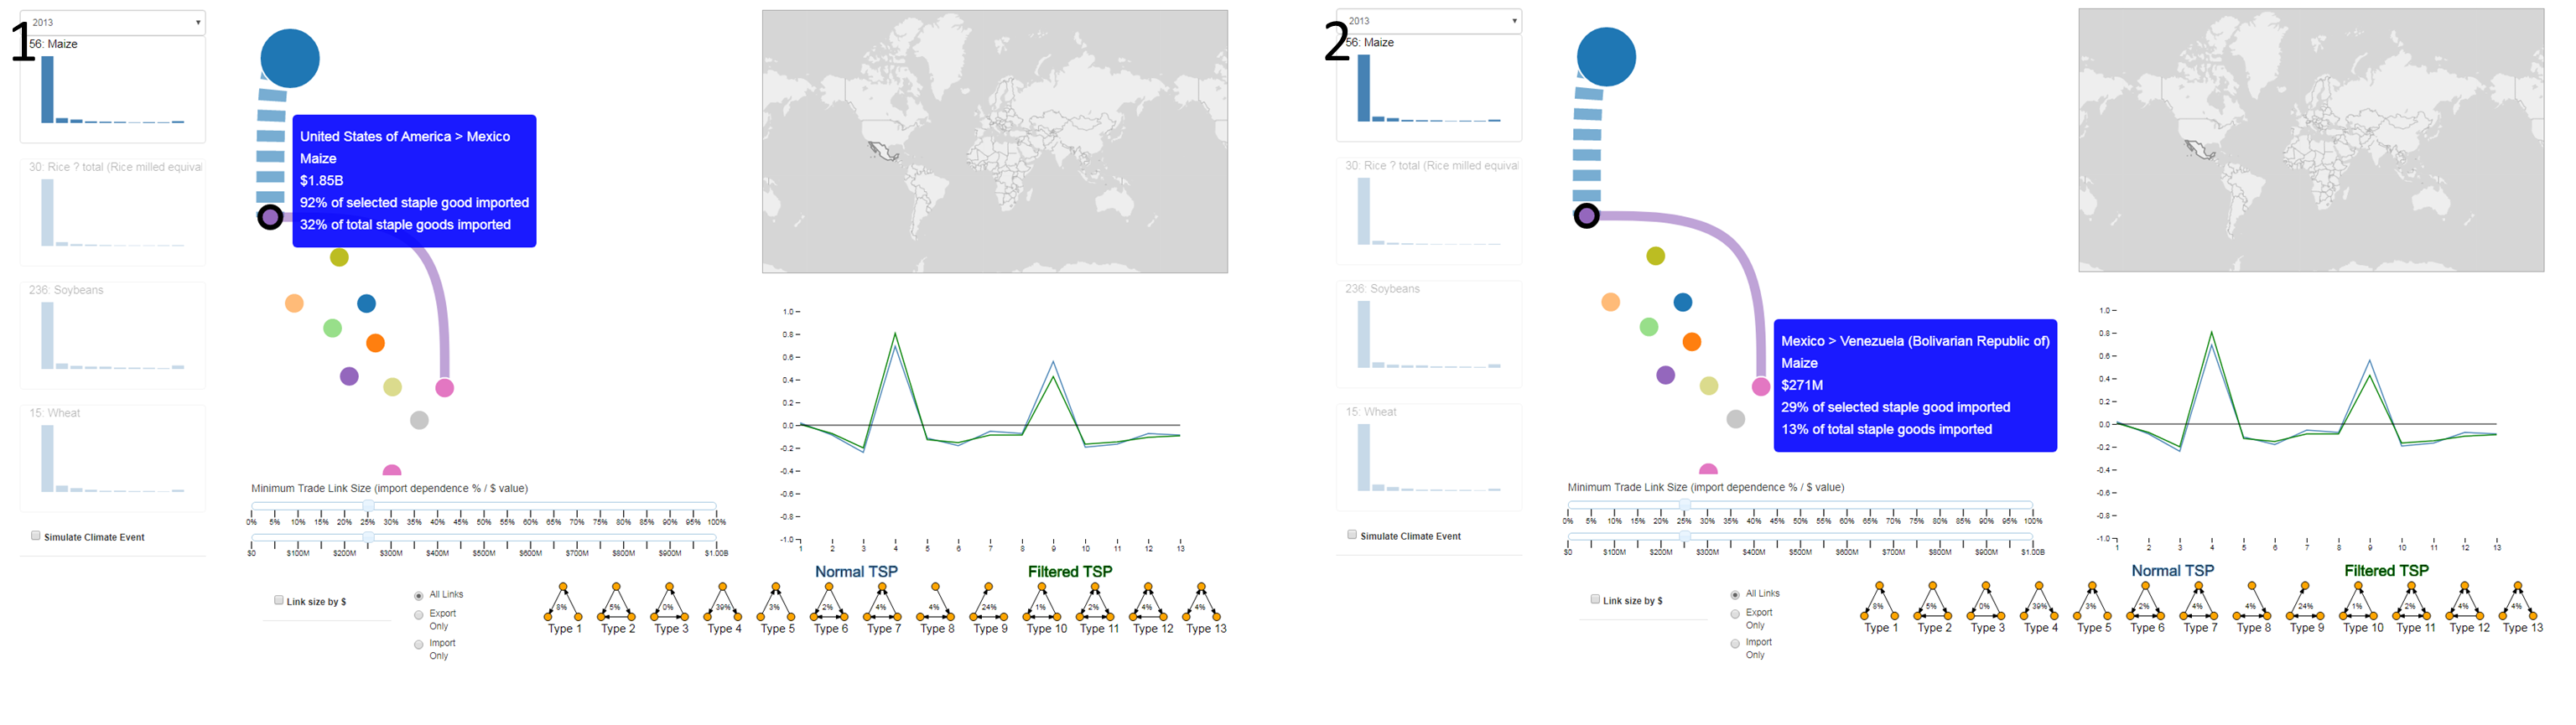
\includegraphics[width=\textwidth]{figures/mexico.png}}
				\caption[MEXICO AS A MIDDLE MAN FOR CORN]{A network graph showing corn that is imported or exported to Mexico(purple). The United States is shown in blue and Venezuela is shown in pink. The network graph has Mexico as the selected country and is filtered to only include export trade links that account for greater than 25\% of the link's importing country's total imports of the trade good. The large dashed line into Mexico shows that Mexico is highly dependent on the United States for a large portion of its corn (92\% from 1, tooltip). The solid line into Venezuela shows that Venezuela is moderately dependent on Mexico for corn (29\% from 2, tooltip).}
				\label{mexicoMiddleMan}
			\end{figure}
		\subsection{Choropleth Map (Section 3, Figure \ref{map})}
		\begin{figure}[htb]
			\center{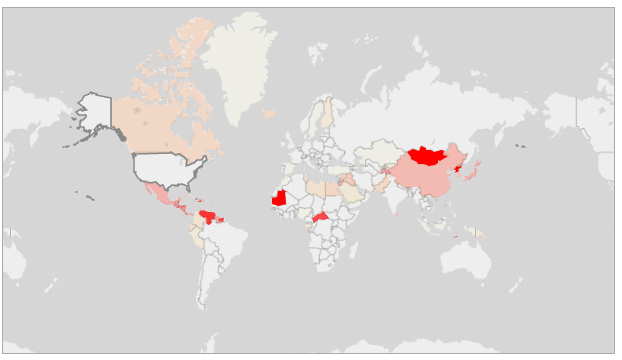
\includegraphics[width=\textwidth]{figures/map.png}}
			\caption[CHOROPLETH MAP OF A SIMULATED UNITED STATES EXPORT REDUCTION]{The choropleth map indicates the impact of a simulated climate event in the selected country on the downstream trade links. In this instance the United States experienced a climate event that reduced the value of corn exports by 10\%. The darker and more red the country is colored, the greater the impact. In this simulation Canada, China, and some central African countries were the most impacted by the event.}
			\label{map}
		\end{figure}
		The choropleth map in Figure \ref{map} shows all countries. The choropleth map is always present, but only colored when a country is selected either here or in the network graph. The positioning in the network graph mirrors the topological layout here to aid in identification of countries without cluttering associated with labels. The choropleth map in Figure \ref{map} gives a visual representation of the vulnerability index by affecting the intensity of coloring based on the loss of imports due to the simulated export reduction from the selected country as defined in Equation \ref{vulnerability}. Anything above 10\% is red and the opacity increases beyond that. If the number of times to cascade is greater than zero, it is possible for the selected country to also be affected. The tooltips in this section show the total imports and exports of the selected good by the country. In the event of a simulation the affected import value, the affected import value to total import ratio, and the affected import value to total trade ratio (Equation \ref{vulnerability}) are also displayed.\par
		The choropleth map is used for identification of vulnerable countries based on the climate event simulated. The more intense and more red the coloring, the higher the vulnerability. \par
		An interesting example of this is Australia. Simulating a 25\% reduction in 2013 wheat exports (Figure \ref{australia}) results in the loss of nearly 95\% of Australia's wheat imports. This is because New Zealand loses \$38 million in wheat trade from Australia and since New Zealand overall exports only \$3 million all trade links are essentially removed in the simulation, including the trade link back to Australia. However, Australia is not colored in heavily in the choropleth map because the loss of the \$600,000 trade link is not a significant percentage of the \$5.79 billion total wheat trade Australia is involved in.\par
		\begin{figure}[htb]
			\center{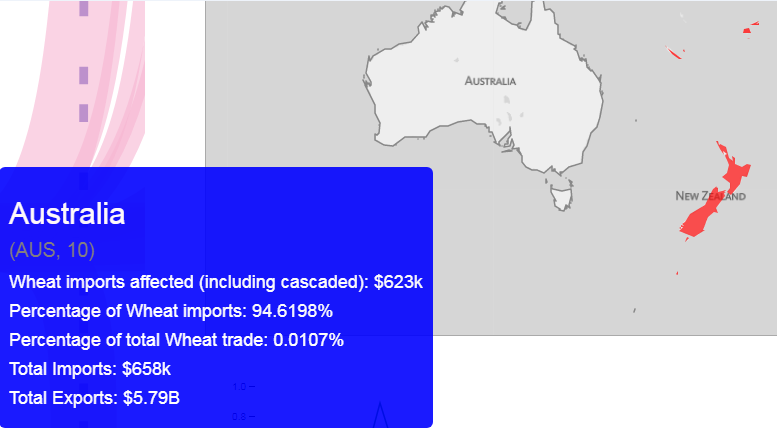
\includegraphics[width=\textwidth]{figures/australia.png}}
			\caption[CHOROPLETH MAP OF A SIMULATED AUSTRALIAN EXPORT REDUCTION]{In this simulation Australia experienced a climate event that reduced the value of wheat exports by 25\%. New Zealand is heavily affected and most of Australia's import links are broken. However, Australia is not colored in heavily in the choropleth map because the loss of the \$600,000 trade link is not a significant percentage of the \$5.79 billion total wheat trade Australia is involved in.}
			\label{australia}
		\end{figure}
	\subsection{Triad Significance Profiles (Section 4, Figures \ref{dashboardSections}-4, \ref{tsps})}
		Figure \ref{dashboardSections}-4 displays a normal triad significance profile (TSP) graph alongside the TSP graph for the current subset of data based on any filtering (e.g. selected country or minimum trade link size). In Figure \ref{dashboardSections}-4 the x-axis in the graph indicates the triad configuration type as shown in Figure \ref{triads}. Figure \ref{triads} shows the 13 different possible configurations in a directed network graph. In Figure \ref{triads} the triad distributions for the network graph of corn in 2013 are also shown. These percentages change based on the current subset of data. The y-axis in Figure \ref{dashboardSections}-4 shows the normalized z-scores defined as
		\begin{equation} \label{zScore}
			z_i=\frac{N^{actual} - N^{random}}{stdev(N^{random})}
		\end{equation}
		where $N^{actual}$ is the actual number of triads of this type and $N^{random}$ is the number of the same type in a randomly generated graph. A positive z-score indicates that the triads occurs more frequently than in a randomly generated network graph, and a negative value less frequently. The blue line shows the normal TSP for all 4 goods across all years of data and the green line is the TSP of the filtered data.\par		
		\begin{figure}[htb]
			\center{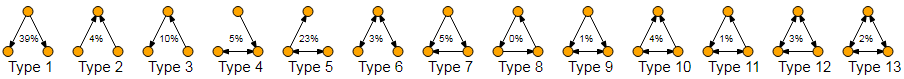
\includegraphics[width=\textwidth]{figures/triads.png}}
			\caption[13 DIFFERENT TRIADS]{The 13 different triads. The percentages here are the distribution of triads for corn in 2013. These values will change with the filtering of data.}
			\label{triads}
		\end{figure}
		Triad significance profiles can aid in the classification and comparison of the network across different types of systems \citep{shutters2012agricultural}. Certain motifs are more or less present in the superfamily identified. Being able to visualize the TSP of the currently filtered data may assist in an assessment of the health of the filtered trade links. Overall, the research in this thesis focused more on cascading impacts to the trade network, but future work will explore the impact of removing network connectors on distributions of triads.\par
		In the data for corn there are some interesting findings. In 1988 (Figure \ref{tsps}, left) we see one dominating triad, type one, which appears a lot more frequently than a random graph would suggest. Note that this triad does not include any bilateral trade links. Progressing from 1988 to 2013, we see the z-score of type nine, ten and thirteen, which all contain bilateral trade links, increase significantly (Figure \ref{triads}, right) and a decrease of type one and two, both unilateral triads. This may indicate an increasingly connected trade network. The increase of type three triads, in which the connecting node acts as a middle man, may suggest the possibility of cascading effects is increased.\par
		\begin{figure}[htb]
			\center{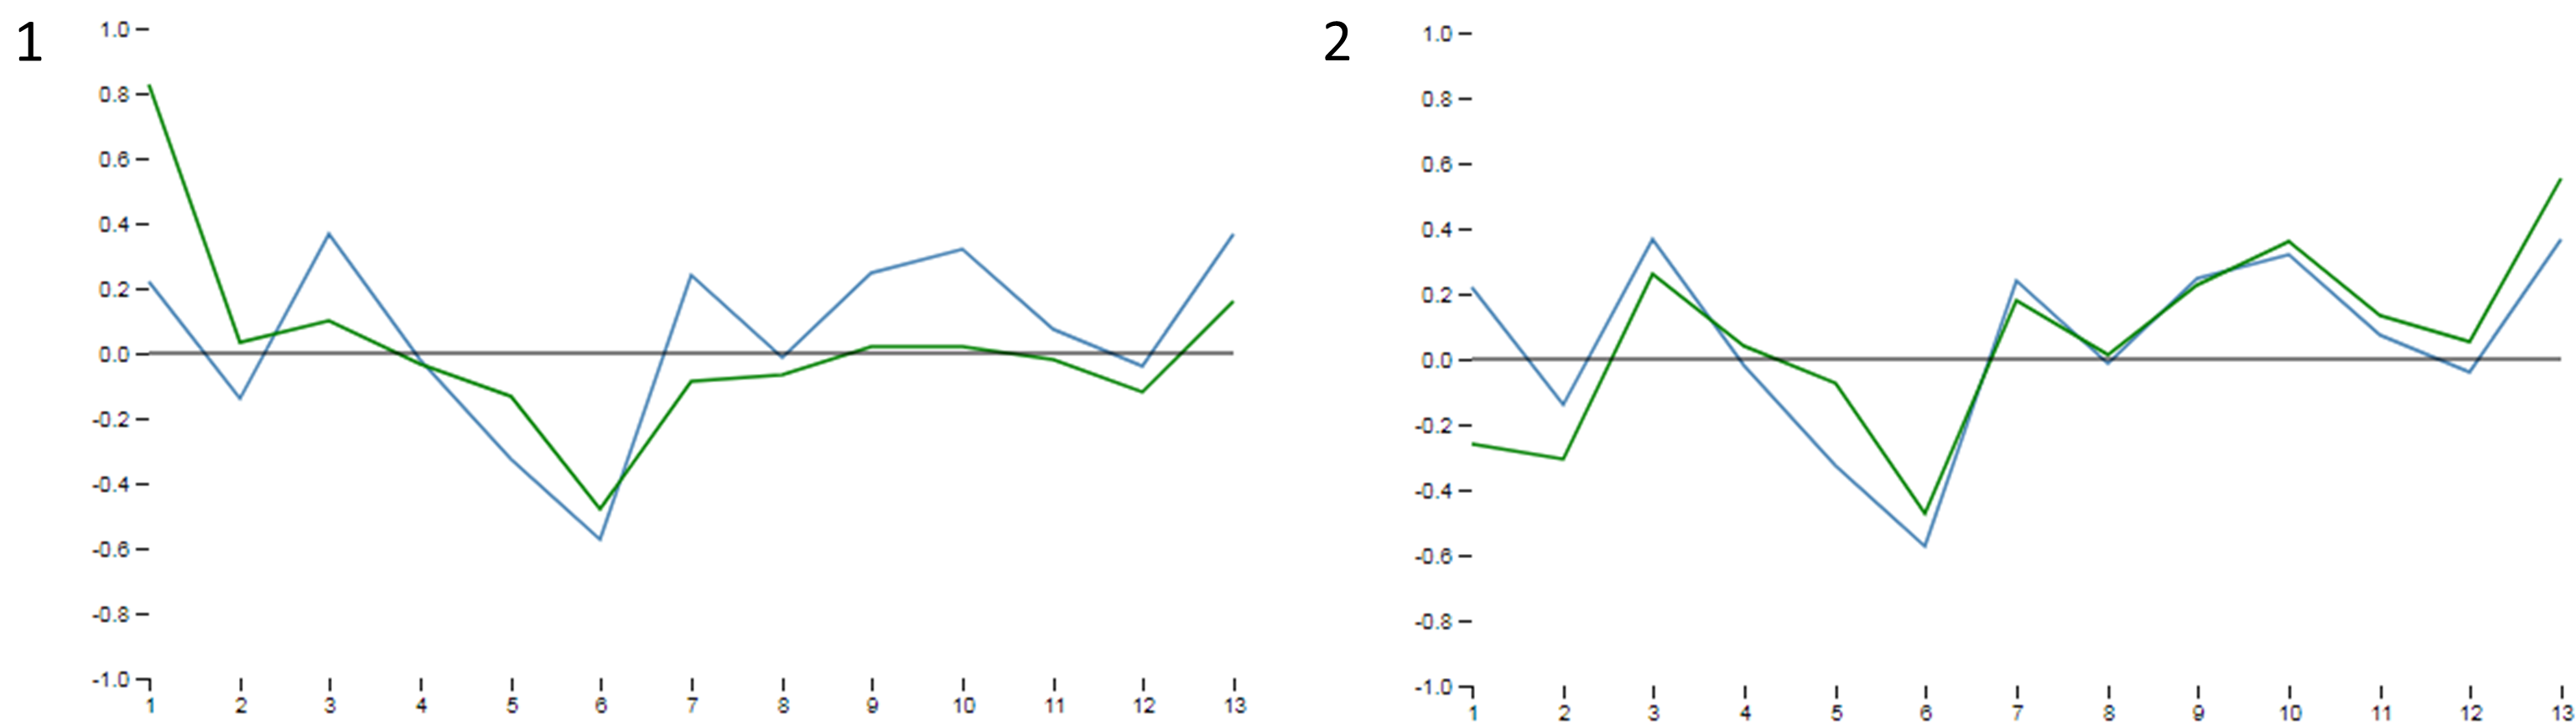
\includegraphics[width=\textwidth]{figures/tsps.png}}
			\caption[TRIAD SIGNIFICANCE PROFILES]{The is a graph that overlays the current triadic significance profile (TSP) with the normal TSP. The graph on the left is the 1988 wheat TSP and the graph on the right is 2013 wheat TSP. }
			\label{tsps}
		\end{figure}
\section{Enhancement Over Existing Visualizations}
	An emphasis of this visual analytics system is the consideration of the global trade network in its entirety. Neither of the reviewed visualizations take into consideration the topology of the food trade network. The FAOSTAT visualization represents only a single point in the food trade network. This does not allow for a direct interpretation of cascading effects. My tool visualizes the entire global trade network. The visualization offered by the Met Office \ref{metOffice} shows an index of food insecurity at a global scale. The focus is on overall vulnerability to food insecurity and does not visualize direct responses to climate events. The interaction and simulated climate events offered by my visual analytic system allow for the exploration of second-order effects of climate events by direct visualization of the affected trade links in the network graph and coloring in the choropleth map.\par
		